\section{Quality Assurance}
\label{sec:quality_assurance}

Software development is more about people, rather than about technologies. That is why there is always a possibility of changing the requirements from the business side or risk of occurring some bug, which can damage the performance of the product because of developer’s mistake. There are many other examples of obstacles, which can appear during the development, but they all have the same issue – they negatively affect the quality of the product. 

Quality is a crucial aspect of every software product. Good quality allows business side to present the product in the best light and successfully compete in the market, because the user always chooses what is the best. Quality cannot be neglected because it will make the product stand out from the rest. So, if the development team tries to save money or time and thus do not pay enough attention to the quality level, then there will definitely appear another team later that will develop almost the same product even cheaper. 

In order to find the balance between all factors during the development process quality assurance techniques should be used. Our team applied different methods for assuring the quality of the SWTcamper. These methods helped us to develop the reliable product and to satisfy customers and clients requirements as much as we could. All quality assurance techniques are listed below.

\subsection{INVEST criteria}
During the project-blastoff our team created a list of user stories regarding to the required functionality for every desired perspective. For this we used project brief, which concise and clearly described requirements which were needed for client and customer.

This process was crucial for us because based on user stories, we planned which functionality should be implemented during each sprint. Also, we derived from the user stories concrete tasks. That is why we used INVEST criteria during the creation of user stories.

Our user stories are \emph{independent} from each other. This means that it allowed team members to implement a valuable working increment for the product without focusing or waiting for finishing another user story.

Our user stories are \emph{negotiable}. Since our team didn’t have enough experience, sometimes we had to rewrite some of our user stories or change acceptance criteria in order to get the desired results by the end of each sprint. We tried to create each user story in such way that there would be enough room for the further discussion between developers and business side, which is good because it gives customer and client opportunity to participate in the development process and to ensure that their requirements were understood correctly.

The next important criteria for user stories is that each user story must be  \emph{valuable}. At the end of each sprint, we had to present a new feature to the customer and client. Without this criterion it would be way harder to determine whether planned workload for the current sprint worth to be showed on the review meeting. We tried to avoid the situation when business side can ask at the end of the review meeting “So what?”. Thus, we tried to implement at first high-priority user stories in order to give business side main functionality as fast as we could.

At the first two sprints we had trouble with estimation the size of user stories. However later, we started to duly appreciate  \emph{estimable} characteristic of each user story. We declared 3 types of size and decided to apply them to every user story we had. So, size L is the biggest one and it corresponds to a quite big volume of work. Roughly, user story with size L took 7 days of work for 2 developers. Aside from size L there was a size M, which corresponds to 5 days of work for 1 developer. And finally, user story with size S took approximately 1-2 days for 1 developer to implement a desired feature. Estimation played a significant role in planning goals for the upcoming sprint because using our custom size we could determine whether will we make it in time or not. 

Our team aimed to create \emph{small} user stories in order to fit in one sprint a few features instead of a gigantic one. We understood that it is more convenient to work with small user stories because it is easier for the whole team to derive concrete tasks and to keep track of development progress in general.

The last but not least, user story must be  \emph{testable}. In order to fulfill this characteristic our team used acceptance criteria. This is a set of test cases which indicates whether our implementation of user story corresponds to requirements or not. If there was a criterion which was uncompleted, then this was a red flag for our team that we had missed something which meant that we should pay extra attention to this case in order to fulfill requirements correctly.

\subsection{SMART criteria}
After the creating user stories by using INVEST criteria, team needed concrete tasks. For deriving tasks from user stories, we decided to use SMART criteria in order to create high-quality tasks. 

Every task must be \emph{specific}. This means that it should be detailed enough for developer, who was assigned to this task. After a few mistakes and misunderstandings inside our team, we figured out how to create a good task. Also, we noticed that such word as “always, never, everywhere, sometimes” signals that the task has not been formulated clearly enough and there may be difficulties in completing or testing the task. 

Developers shall understand when the task is done. That is why characteristic \emph{measurable} is essential for every task. Since team members had had different skill level it was crucial to formalize task in that way that every developer could understand whether task was done correctly. 

At the beginning of the module, we faced the fact that our tasks are huge, and it takes ages to complete them which is not fine because of  \emph{achievability}. As mentioned before developers had different skill backgrounds and that is why it was very important to create task, which could be completed within sprint and with reasonable complexity. 

Also, at the beginning and at the end our understanding to a task management differs. At first, we tried to separate tasks by the type (backend, frontend, bug fixing) and assign tasks separately to each team member according to his/her preferences in order to fully concentrate on the given issue. However, after a while we started to combine different types of functionality of the concrete feature into one task and to assign such task instead of one to two team members. We found out that it was much better to have specification of desired feature in one task and two students from our team could implement this faster as these tasks were separated. 

Say, it was a good decision to assign to three students task, which says, that they must create UI for login view, controller as well as operations with database in a one single task. Even experienced developer can stack during developing such task alone but our mini-team accomplished this task in a good manner.  

It was crucial for the team to use the given time for developing SWTcamper as much effective as it was possible because of the lack of working time. That is why everyone wanted to complete only \emph{relevant} tasks. The more relevant tasks were done the more our team could achieve during the development process.

Of course, programming can be extremely fascinating, and it gives developers opportunity to complete every task in many creative ways (especially UI), but business side always expects working product on time. That is why we tried to make every task \emph{time-boxed} in order to make the whole product on time. However, due to the lack of time and complexity of this management activity almost no one could properly define the deadline and make a correct time tracking. Our team decided to focus on the other aspects. However, we still had for every sprint rough plan with planned features to implement and if there were any issues during the implementing one more team member was assigned to the task.  

\subsection{Reviews}
There are a lot of types of review, but our team chose the informal one due to time limits and simplification of the review-process. Suppose developer completed the task and he/she wants to merge it to the dev branch. In order to mitigate the risks of appearing of merge conflicts or incorrect implementation, developer should first of all notify team members that the task is done and now it is waiting for review. 

Reviewer shall carefully check source code which was written for the upcoming merge-request and if he/she spots any issue in the code it has to be commented. Thus, we have strived to create a discussion about problem case in order to fix this as fast as it was possible and to make sure that the developer who accidently produced code with issue did not lose motivation to move on and finish the project.   

At the beginning of the module, we had a problem with our merge requests because we did not have the correct understanding of how to work with code as a team. That is why sometimes we had to meet all together and provide walkthroughs in the code before merging in the dev branch. This type of meetings was more formal for us but still we did not see sense in additional documentation. However, we had a checklist for every walkthrough in order to effectively use time and we had also a volunteer who was a moderator of such meeting. Although these walkthroughs were helpful, they were time consuming and a bit stressful. That is why our team was happy when we learned how to complete assigned tasks correctly and without merge-conflicts.

\subsection{Testing}
One more quality assurance technique which we have used was testing. Although testing is not an ideal method for ensuring that our product works without errors, we still can find out presence of them. Since our team was well aware about inner workings of the application, we mainly used white-box testing. 

\emph{Unit testing} allowed us to test a given class in isolated environment in order to ensure that its logic corresponds to requirements. Of course, it was impossible to test every case. That is why team tried to test mainly “corner-cases”, but we also have test with “normal” parameters.  Since we wanted to test concrete class, we should use mocking-functionality to create stubs for methods from other classes.

\emph{Integration testing} gave us opportunity to check whether our classes work without errors together. It was a pivotal part of the testing because it mitigated risks of occurring merge conflicts. Although this technique was useful, it was quite challenging to create a lot of integration tests because of their complexity.

For \emph{test coverage} our team decided to use basic functionality of IDE IntelliJ. We agreed that sufficient percentage of coverage shall be 80\% for all service-classes.

Although we have not created tests for frontend, we still tested it manually to avoid errors in the UI.

\subsection{Pipeline}
Before creating a merge-request author should ensure that his/her code corresponds to agreed conventions. For this our team used pipeline offered by SWT chair. 

Our pipeline consists of 3 stages. First stage actively uses java code formatter. So, this stage rewrites our code with attention to the maximum line length. Second stage checked code’s ability to compile and the last one ran all tests to ensure that they all work perfectly fine. If any of stages fails, then the whole pipeline fails, which meant that the given code couldn’t be merged in the way it was presented to pipeline. We used it as, say, self-check before presenting our implementation to other team members.

Pipeline helped us to automatically check all necessary aspects of successful merge procedure. Because of the lack of experience team members made sometimes mistakes and pipeline helped us to detect them. Also, running a pipeline was way faster than to gather whole our team together to detect errors in code.  Of course, it did not make the whole work instead of us, but it was still a good tool to use.  

\subsection{Pair programming}
At the beginning of the module everyone had his/her own task to work with. Over time we figured out that working in pairs increases our overall efficiency. 

This method of task completing saved us a lot of time and kept our moral up. It matters when team members know that they can rely on each other in a way that they can always ask a question or ask to prompt how to resolve the issue. 

Also, pair programming increases discipline inside of the team which positively impacts on the quality of the product.  Different experience level is only plus in terms of scrum development. Pair programming allows team members to share tricks and healthy design patterns between each other which makes code definitely better.

\subsection{Prototyping}
At the project blastoff it was crucial for the whole team to understand what we all were going to build. We had a project brief, and we wrote down user stories. But for the “full picture” we needed a prototype of the application. It was relatively fast to implement and required way less skill set than programming. 

We made our prototype in the PowerPoint and showed it on the first review meeting. Business side was satisfied with our vision of the product. Also, prototype helped us to refine and even elicit additional requirements for the product. Additionally, prototyping is one of the best techniques to find the most appropriate user interface and to show team members how the product will work not only under the hood but also for the regular users.

\subsection{Feedback from business side}
In order to fulfill all the requirements from customer and client our team attended review meetings as well as PO-meetings. We have understood how it was important to communicate with business side throughout the whole development process. It was extremely hard to define everything in documentation at once and that is why frequent meetings were very helpful.

Review meetings gave us the opportunity to assess our current progress basing on the reaction of client and customer. Also, we tried to gather all possible information about wishes and plans of the business in order to implement the most valuable features in the application as fast as we can.

PO meetings were used mainly to refine the requirements and to eliminate any possible ambiguities regarding implementation. Often PO meetings corrected our understanding regarding some features which helped us to synchronize with requirements from the business side.

\subsection{Normalization}
While designing our database, we realized that we have to stick to methods which will allow us to correctly organize data in database. We decided that normalization was the most relevant to us. Main principles which we have used were eliminating redundancy and inconsistent dependencies in our database.

Redundant data will create difficulties while maintaining the application in future. Also, redundant data is space-consuming which means additional costs for the business side. 

Inconsistent data makes difficult data to access and evaluate because of broken path in the database. It will be time consuming to reorganize database in right way in future as well as to provide analysis for given data.

In order to avoid such issues, we designed our database with respect to normalization rules. That is why our database is in the “third normal form”. Our database does not have repeating groups in every table, it has a separate table for each set of related data which also has only one primary key. It worth mentioning that each non-primary attribute in every table depends on the primary key of entities. 

\subsection{Summary}
Our team was trying to implement application with respect to different quality assurance techniques. It helped us to improve level of quality of our product and also, we have understood how to improve the workflow inside the team as well as how to establish informative conversation with business side. The figure below presents all quality assurance techniques that our team have used during the module.

\begin{figure}[h]
    \centering
    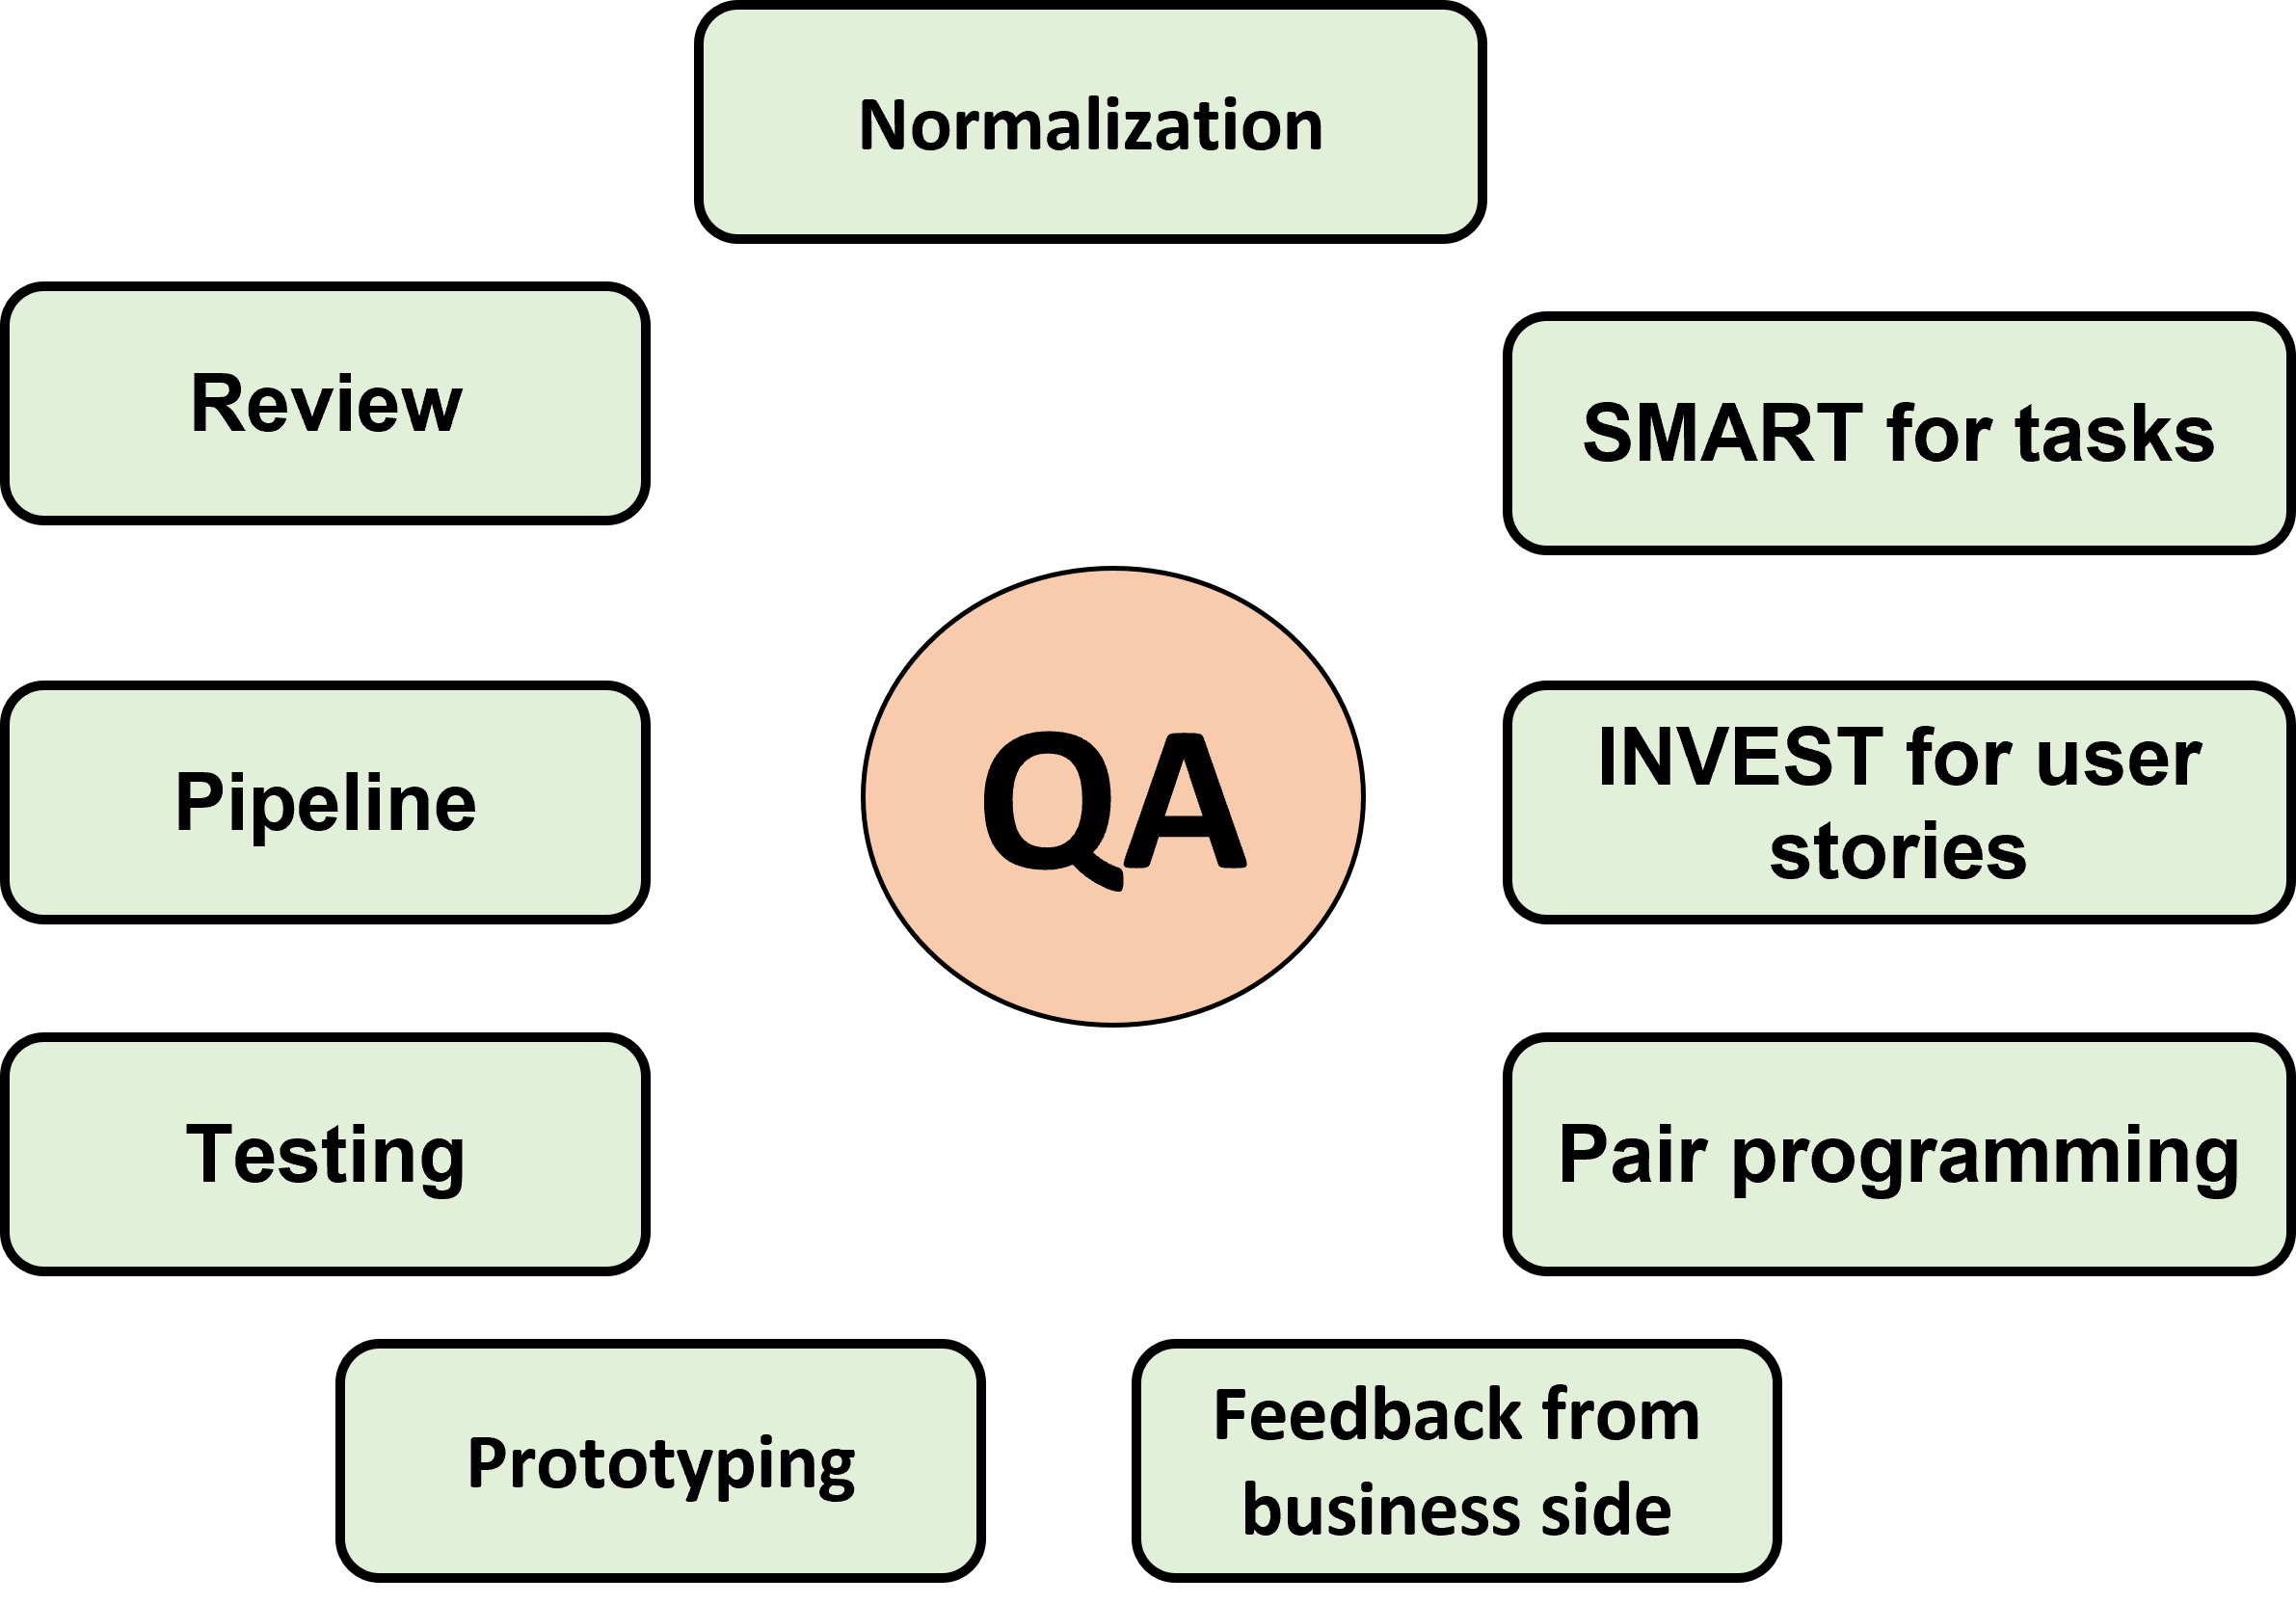
\includegraphics[scale=0.75]{resources/images/qa-techniques.png}
    \caption{QA techniques}
    \label{fig:qa-techniques}
\end{figure}